\documentclass[a4paper]{article}

%% Language and font encodings
\usepackage[english]{babel}
\usepackage[utf8x]{inputenc}
\usepackage[T1]{fontenc}

%% Sets page size and margins
\usepackage[a4paper,top=3cm,bottom=2cm,left=3cm,right=3cm,marginparwidth=1.75cm]{geometry}

%% Useful packages
\usepackage{amsmath}
\usepackage{graphicx}
\usepackage[colorinlistoftodos]{todonotes}
\usepackage[colorlinks=true, allcolors=blue]{hyperref}


\title{Developing Chess in Lua}
\author{Cameron Wright, Maddie Ross, Spencer Saunders}

\begin{document}
\maketitle

\begin{abstract}
This paper goes over the proposal of developing Chess using the programming language Lua.  Lua is a scripting language but also is object-oriented, these attributes will help us in designing Chess in a modular fashion.  The final solution should be a game of Chess playable from one computer between two people with a simple interface.  
\end{abstract}

\section{Introduction}

\subsection{Why Chess?}
For our programming language project, we decided to go with developing Chess in Lua. Chess is a universally popular game, and because of how popular it is, we figured it'd be our best option for creating a game given how many resources are available online that describe the various rules and plays of chess that will help aid us if we run into any roadblocks. 

An additional reason why we went with this project is we have a lot of flexibility in regard to how we implement the chess game whether it's using a GUI or ASCII output to the console to simulate a chess game.

Finally, we decided to go with chess as our final project because it'll be a challenging project but it won't be biting off more than we can chew. Developing a chess game is a doable process that'll require quite a bit of work but it won't have us rushing to reach the deadline with an overabundance of work.

\begin{figure}
\centering
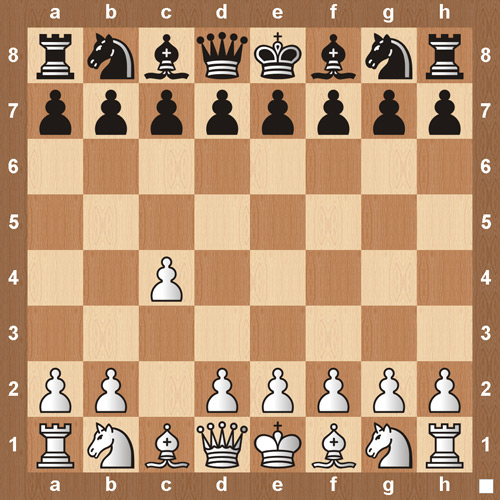
\includegraphics[width=0.3\textwidth]{chessboard.jpg}
\caption{\label{fig:Chess}A standard Chess board.}
\end{figure}

\subsection{Our idea}
The chess game we will be creating will be one-on-one. We will not be implementing a bot-version of the chess game where one user plays against an AI. We felt that implementing a bot in our project would be biting off more than we can chew and that it'd be best to stick solely to a PvP (player vs. player) game mode. 

\section{Project Description}

Chess as a game has defined rules and is complex enough to require thought.  Chess is a game between two people moving Chess pieces on a board trying to strategically take out the others king Figure represented in Figure \ref{fig:Chess}.  Lua is a scripting language, and "supports procedural programming, object-oriented programming, functional programming, data-driven programming, and data description" \cite{Lua}.  As a language that allows object-oriented principles, Lua allow us to define what a board, piece, and a game is.  A piece would be an abstract class that all different pieces like king, queen, pawn, rook inherit from as sub classes.  A board would be an object containing pieces and what is allowed and not when moving pieces.  Lastly a way to display the board would be needed for two players to play on one computer.  The window or board would be displayed using ASCII characters though using minimal coupling, swapping out different types of windows for something like a GUI would be easier.  Some challenges that will be faced when designing Chess will come with where we want to handle certain operations, for example would available moves a Chess piece can take be calculated on the board or within the Chess piece class.

\section{Evaluation}

Evaluating the current state of the project will be based on the current working state of the game for players and the current bugs within the game.  Chess and the pieces have lot of different combinations and states that they can be in.  Instead of testing for every different combination the pieces on the board can be, a focus will be on legal moves vs illegal moves and making sure that no move breaks the game or is allowed.  The game will be behave more as a state machine where the game is either starting, being played, or just finishing.

\section{Management}

\subsection{Mile Stones}

\begin{enumerate}
\item Define board and piece framework.
\item Design game logic and rules.
\item Build driver that will run game.
\item Test and debug project.
\item Finish game and play with ASCII board.
\end{enumerate}

\subsection{Group Communication}

Communicating as a group is important to delegate tasks.  The team will be using a Trello board for showing current tasks.  For storing the project GitHub will be used as source control.  Table Table \ref{tab:contacts} Shows email to contact all team members.

\begin{table*}[ht]
\centering
\small
 \begin{tabular}{r|c}
\hline
\textbf{Name} & \textbf{Email}\\
\hline
\textbf{Cameron Wright}  & cameronwright@u.boisestate   \\
\textbf{Maddie Ross}    & maddieross@u.boisestate.edu   \\
\textbf{Spencer Saunders}    & spencersaunders@u.boisestate.edu  \\
\end{tabular}
\caption{Names and emails}
\label{tab:contacts}
\end{table*}

\subsection{Individual Contributions}

We have not yet decided who is going to do what. It will be an on-going process where we'll mock-up a design for the project, designate who does what, and he will have weekly check-ins to ensure that everything is being accounted for and finished. 

\bibliographystyle{alpha}
\bibliography{sample}

\end{document}